\documentclass[1p]{elsarticle_modified}
%\bibliographystyle{elsarticle-num}

%\usepackage[colorlinks]{hyperref}
%\usepackage{abbrmath_seonhwa} %\Abb, \Ascr, \Acal ,\Abf, \Afrak
\usepackage{amsfonts}
\usepackage{amssymb}
\usepackage{amsmath}
\usepackage{amsthm}
\usepackage{scalefnt}
\usepackage{amsbsy}
\usepackage{kotex}
\usepackage{caption}
\usepackage{subfig}
\usepackage{color}
\usepackage{graphicx}
\usepackage{xcolor} %% white, black, red, green, blue, cyan, magenta, yellow
\usepackage{float}
\usepackage{setspace}
\usepackage{hyperref}

\usepackage{tikz}
\usetikzlibrary{arrows}

\usepackage{multirow}
\usepackage{array} % fixed length table
\usepackage{hhline}

%%%%%%%%%%%%%%%%%%%%%
\makeatletter
\renewcommand*\env@matrix[1][\arraystretch]{%
	\edef\arraystretch{#1}%
	\hskip -\arraycolsep
	\let\@ifnextchar\new@ifnextchar
	\array{*\c@MaxMatrixCols c}}
\makeatother %https://tex.stackexchange.com/questions/14071/how-can-i-increase-the-line-spacing-in-a-matrix
%%%%%%%%%%%%%%%

\usepackage[normalem]{ulem}

\newcommand{\msout}[1]{\ifmmode\text{\sout{\ensuremath{#1}}}\else\sout{#1}\fi}
%SOURCE: \msout is \stkout macro in https://tex.stackexchange.com/questions/20609/strikeout-in-math-mode

\newcommand{\cancel}[1]{
	\ifmmode
	{\color{red}\msout{#1}}
	\else
	{\color{red}\sout{#1}}
	\fi
}

\newcommand{\add}[1]{
	{\color{blue}\uwave{#1}}
}

\newcommand{\replace}[2]{
	\ifmmode
	{\color{red}\msout{#1}}{\color{blue}\uwave{#2}}
	\else
	{\color{red}\sout{#1}}{\color{blue}\uwave{#2}}
	\fi
}

\newcommand{\Sol}{\mathcal{S}} %segment
\newcommand{\D}{D} %diagram
\newcommand{\A}{\mathcal{A}} %arc


%%%%%%%%%%%%%%%%%%%%%%%%%%%%%5 test

\def\sl{\operatorname{\textup{SL}}(2,\Cbb)}
\def\psl{\operatorname{\textup{PSL}}(2,\Cbb)}
\def\quan{\mkern 1mu \triangleright \mkern 1mu}

\theoremstyle{definition}
\newtheorem{thm}{Theorem}[section]
\newtheorem{prop}[thm]{Proposition}
\newtheorem{lem}[thm]{Lemma}
\newtheorem{ques}[thm]{Question}
\newtheorem{cor}[thm]{Corollary}
\newtheorem{defn}[thm]{Definition}
\newtheorem{exam}[thm]{Example}
\newtheorem{rmk}[thm]{Remark}
\newtheorem{alg}[thm]{Algorithm}

\newcommand{\I}{\sqrt{-1}}
\begin{document}

%\begin{frontmatter}
%
%\title{Boundary parabolic representations of knots up to 8 crossings}
%
%%% Group authors per affiliation:
%\author{Yunhi Cho} 
%\address{Department of Mathematics, University of Seoul, Seoul, Korea}
%\ead{yhcho@uos.ac.kr}
%
%
%\author{Seonhwa Kim} %\fnref{s_kim}}
%\address{Center for Geometry and Physics, Institute for Basic Science, Pohang, 37673, Korea}
%\ead{ryeona17@ibs.re.kr}
%
%\author{Hyuk Kim}
%\address{Department of Mathematical Sciences, Seoul National University, Seoul 08826, Korea}
%\ead{hyukkim@snu.ac.kr}
%
%\author{Seokbeom Yoon}
%\address{Department of Mathematical Sciences, Seoul National University, Seoul, 08826,  Korea}
%\ead{sbyoon15@snu.ac.kr}
%
%\begin{abstract}
%We find all boundary parabolic representation of knots up to 8 crossings.
%
%\end{abstract}
%\begin{keyword}
%    \MSC[2010] 57M25 
%\end{keyword}
%
%\end{frontmatter}

%\linenumbers
%\tableofcontents
%
\newcommand\colored[1]{\textcolor{white}{\rule[-0.35ex]{0.8em}{1.4ex}}\kern-0.8em\color{red} #1}%
%\newcommand\colored[1]{\textcolor{white}{ #1}\kern-2.17ex	\textcolor{white}{ #1}\kern-1.81ex	\textcolor{white}{ #1}\kern-2.15ex\color{red}#1	}

{\Large $\underline{12a_{0250}~(K12a_{0250})}$}

\setlength{\tabcolsep}{10pt}
\renewcommand{\arraystretch}{1.6}
\vspace{1cm}\begin{tabular}{m{100pt}>{\centering\arraybackslash}m{274pt}}
\multirow{5}{120pt}{
	\centering
	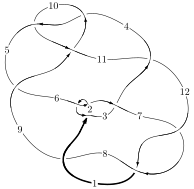
\includegraphics[width=112pt]{../../../GIT/diagram.site/Diagrams/png/1051_12a_0250.png}\\
\ \ \ A knot diagram\footnotemark}&
\allowdisplaybreaks
\textbf{Linearized knot diagam} \\
\cline{2-2}
 &
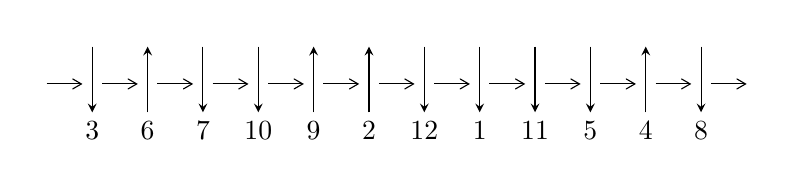
\begin{tikzpicture}[x=20pt, y=17pt]
	% nodes
	\node (C0) at (0, 0) {};
	\node (C1) at (1, 0) {};
	\node (C1U) at (1, +1) {};
	\node (C1D) at (1, -1) {3};

	\node (C2) at (2, 0) {};
	\node (C2U) at (2, +1) {};
	\node (C2D) at (2, -1) {6};

	\node (C3) at (3, 0) {};
	\node (C3U) at (3, +1) {};
	\node (C3D) at (3, -1) {7};

	\node (C4) at (4, 0) {};
	\node (C4U) at (4, +1) {};
	\node (C4D) at (4, -1) {10};

	\node (C5) at (5, 0) {};
	\node (C5U) at (5, +1) {};
	\node (C5D) at (5, -1) {9};

	\node (C6) at (6, 0) {};
	\node (C6U) at (6, +1) {};
	\node (C6D) at (6, -1) {2};

	\node (C7) at (7, 0) {};
	\node (C7U) at (7, +1) {};
	\node (C7D) at (7, -1) {12};

	\node (C8) at (8, 0) {};
	\node (C8U) at (8, +1) {};
	\node (C8D) at (8, -1) {1};

	\node (C9) at (9, 0) {};
	\node (C9U) at (9, +1) {};
	\node (C9D) at (9, -1) {11};

	\node (C10) at (10, 0) {};
	\node (C10U) at (10, +1) {};
	\node (C10D) at (10, -1) {5};

	\node (C11) at (11, 0) {};
	\node (C11U) at (11, +1) {};
	\node (C11D) at (11, -1) {4};

	\node (C12) at (12, 0) {};
	\node (C12U) at (12, +1) {};
	\node (C12D) at (12, -1) {8};
	\node (C13) at (13, 0) {};

	% arrows
	\draw[->,>={angle 60}]
	(C0) edge (C1) (C1) edge (C2) (C2) edge (C3) (C3) edge (C4) (C4) edge (C5) (C5) edge (C6) (C6) edge (C7) (C7) edge (C8) (C8) edge (C9) (C9) edge (C10) (C10) edge (C11) (C11) edge (C12) (C12) edge (C13) ;	\draw[->,>=stealth]
	(C1U) edge (C1D) (C2D) edge (C2U) (C3U) edge (C3D) (C4U) edge (C4D) (C5D) edge (C5U) (C6D) edge (C6U) (C7U) edge (C7D) (C8U) edge (C8D) (C9U) edge (C9D) (C10U) edge (C10D) (C11D) edge (C11U) (C12U) edge (C12D) ;
	\end{tikzpicture} \\
\hhline{~~} \\& 
\textbf{Solving Sequence} \\ \cline{2-2} 
 &
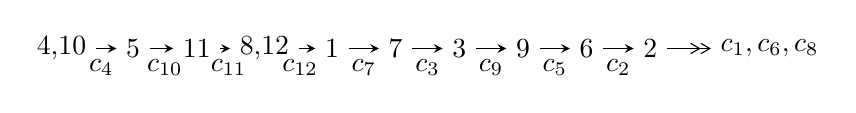
\begin{tikzpicture}[x=23pt, y=7pt]
	% node
	\node (A0) at (-1/8, 0) {4,10};
	\node (A1) at (1, 0) {5};
	\node (A2) at (2, 0) {11};
	\node (A3) at (49/16, 0) {8,12};
	\node (A4) at (33/8, 0) {1};
	\node (A5) at (41/8, 0) {7};
	\node (A6) at (49/8, 0) {3};
	\node (A7) at (57/8, 0) {9};
	\node (A8) at (65/8, 0) {6};
	\node (A9) at (73/8, 0) {2};
	\node (C1) at (1/2, -1) {$c_{4}$};
	\node (C2) at (3/2, -1) {$c_{10}$};
	\node (C3) at (5/2, -1) {$c_{11}$};
	\node (C4) at (29/8, -1) {$c_{12}$};
	\node (C5) at (37/8, -1) {$c_{7}$};
	\node (C6) at (45/8, -1) {$c_{3}$};
	\node (C7) at (53/8, -1) {$c_{9}$};
	\node (C8) at (61/8, -1) {$c_{5}$};
	\node (C9) at (69/8, -1) {$c_{2}$};
	\node (A10) at (11, 0) {$c_{1},c_{6},c_{8}$};

	% edge
	\draw[->,>=stealth]	
	(A0) edge (A1) (A1) edge (A2) (A2) edge (A3) (A3) edge (A4) (A4) edge (A5) (A5) edge (A6) (A6) edge (A7) (A7) edge (A8) (A8) edge (A9) ;
	\draw[->>,>={angle 60}]	
	(A9) edge (A10);
\end{tikzpicture} \\ 

\end{tabular} \\

\footnotetext{
The image of knot diagram is generated by the software ``\textbf{Draw programme}" developed by Andrew Bartholomew(\url{http://www.layer8.co.uk/maths/draw/index.htm\#Running-draw}), where we modified some parts for our purpose(\url{https://github.com/CATsTAILs/LinksPainter}).
}\phantom \\ \newline 
\centering \textbf{Ideals for irreducible components\footnotemark of $X_{\text{par}}$} 
 
\begin{align*}
I^u_{1}&=\langle 
-1.19066\times10^{46} u^{91}-8.76887\times10^{45} u^{90}+\cdots+1.29375\times10^{46} b-2.58000\times10^{46},\\
\phantom{I^u_{1}}&\phantom{= \langle  }-1.24081\times10^{46} u^{91}-6.18183\times10^{45} u^{90}+\cdots+1.29375\times10^{46} a-1.65575\times10^{46},\;u^{92}- u^{91}+\cdots-4 u-4\rangle \\
I^u_{2}&=\langle 
- u^2 a- u^3+2 b+u,\;-2 u^3 a-2 u^2 a+2 a^2-3 u^2+4 a-2 u+2,\;u^4-2 u^2+2\rangle \\
\\
I^v_{1}&=\langle 
a,\;b- v-1,\;v^2+v+1\rangle \\
\end{align*}
\raggedright * 3 irreducible components of $\dim_{\mathbb{C}}=0$, with total 102 representations.\\
\footnotetext{All coefficients of polynomials are rational numbers. But the coefficients are sometimes approximated in decimal forms when there is not enough margin.}
\newpage
\renewcommand{\arraystretch}{1}
\centering \section*{I. $I^u_{1}= \langle -1.19\times10^{46} u^{91}-8.77\times10^{45} u^{90}+\cdots+1.29\times10^{46} b-2.58\times10^{46},\;-1.24\times10^{46} u^{91}-6.18\times10^{45} u^{90}+\cdots+1.29\times10^{46} a-1.66\times10^{46},\;u^{92}- u^{91}+\cdots-4 u-4 \rangle$}
\flushleft \textbf{(i) Arc colorings}\\
\begin{tabular}{m{7pt} m{180pt} m{7pt} m{180pt} }
\flushright $a_{4}=$&$\begin{pmatrix}1\\0\end{pmatrix}$ \\
\flushright $a_{10}=$&$\begin{pmatrix}0\\u\end{pmatrix}$ \\
\flushright $a_{5}=$&$\begin{pmatrix}1\\u^2\end{pmatrix}$ \\
\flushright $a_{11}=$&$\begin{pmatrix}- u\\- u^3+u\end{pmatrix}$ \\
\flushright $a_{8}=$&$\begin{pmatrix}0.959085 u^{91}+0.477824 u^{90}+\cdots+1.76621 u+1.27981\\0.920318 u^{91}+0.677789 u^{90}+\cdots-0.789492 u+1.99421\end{pmatrix}$ \\
\flushright $a_{12}=$&$\begin{pmatrix}- u^3\\- u^3+u\end{pmatrix}$ \\
\flushright $a_{1}=$&$\begin{pmatrix}-0.959085 u^{91}-0.477824 u^{90}+\cdots-1.76621 u-1.27981\\-0.520135 u^{91}+0.568999 u^{90}+\cdots-10.3735 u-3.75342\end{pmatrix}$ \\
\flushright $a_{7}=$&$\begin{pmatrix}2.25174 u^{91}+0.140564 u^{90}+\cdots+13.7323 u+6.98810\\0.648520 u^{91}+0.477914 u^{90}+\cdots+0.939846 u+2.00720\end{pmatrix}$ \\
\flushright $a_{3}=$&$\begin{pmatrix}-2.40424 u^{91}+0.353032 u^{90}+\cdots-17.0716 u-7.38408\\-2.56979 u^{91}+0.701142 u^{90}+\cdots-26.3860 u-11.8827\end{pmatrix}$ \\
\flushright $a_{9}=$&$\begin{pmatrix}u^3\\u^5- u^3+u\end{pmatrix}$ \\
\flushright $a_{6}=$&$\begin{pmatrix}u^6- u^4+1\\u^8-2 u^6+2 u^4\end{pmatrix}$ \\
\flushright $a_{2}=$&$\begin{pmatrix}-1.85644 u^{91}+0.247883 u^{90}+\cdots-14.9023 u-6.27237\\-2.07702 u^{91}+0.589387 u^{90}+\cdots-21.4547 u-9.72321\end{pmatrix}$\\&\end{tabular}
\flushleft \textbf{(ii) Obstruction class $= -1$}\\~\\
\flushleft \textbf{(iii) Cusp Shapes $= 2.70406 u^{91}-2.77366 u^{90}+\cdots+10.6535 u-2.61646$}\\~\\
\newpage\renewcommand{\arraystretch}{1}
\flushleft \textbf{(iv) u-Polynomials at the component}\newline \\
\begin{tabular}{m{50pt}|m{274pt}}
Crossings & \hspace{64pt}u-Polynomials at each crossing \\
\hline $$\begin{aligned}c_{1}\end{aligned}$$&$\begin{aligned}
&u^{92}+48 u^{91}+\cdots+34 u+25
\end{aligned}$\\
\hline $$\begin{aligned}c_{2},c_{6}\end{aligned}$$&$\begin{aligned}
&u^{92}-2 u^{91}+\cdots+4 u+5
\end{aligned}$\\
\hline $$\begin{aligned}c_{3}\end{aligned}$$&$\begin{aligned}
&u^{92}+2 u^{91}+\cdots+27428 u+5585
\end{aligned}$\\
\hline $$\begin{aligned}c_{4},c_{10}\end{aligned}$$&$\begin{aligned}
&u^{92}- u^{91}+\cdots-4 u-4
\end{aligned}$\\
\hline $$\begin{aligned}c_{5},c_{11}\end{aligned}$$&$\begin{aligned}
&u^{92}-3 u^{91}+\cdots-1388 u+172
\end{aligned}$\\
\hline $$\begin{aligned}c_{7},c_{8},c_{12}\end{aligned}$$&$\begin{aligned}
&u^{92}+3 u^{91}+\cdots+21 u-1
\end{aligned}$\\
\hline $$\begin{aligned}c_{9}\end{aligned}$$&$\begin{aligned}
&u^{92}+51 u^{91}+\cdots+80 u+16
\end{aligned}$\\
\hline
\end{tabular}\\~\\
\newpage\renewcommand{\arraystretch}{1}
\flushleft \textbf{(v) Riley Polynomials at the component}\newline \\
\begin{tabular}{m{50pt}|m{274pt}}
Crossings & \hspace{64pt}Riley Polynomials at each crossing \\
\hline $$\begin{aligned}c_{1}\end{aligned}$$&$\begin{aligned}
&y^{92}+96 y^{90}+\cdots-56506 y+625
\end{aligned}$\\
\hline $$\begin{aligned}c_{2},c_{6}\end{aligned}$$&$\begin{aligned}
&y^{92}+48 y^{91}+\cdots+34 y+25
\end{aligned}$\\
\hline $$\begin{aligned}c_{3}\end{aligned}$$&$\begin{aligned}
&y^{92}-48 y^{91}+\cdots+824383826 y+31192225
\end{aligned}$\\
\hline $$\begin{aligned}c_{4},c_{10}\end{aligned}$$&$\begin{aligned}
&y^{92}-51 y^{91}+\cdots-80 y+16
\end{aligned}$\\
\hline $$\begin{aligned}c_{5},c_{11}\end{aligned}$$&$\begin{aligned}
&y^{92}+81 y^{91}+\cdots-825744 y+29584
\end{aligned}$\\
\hline $$\begin{aligned}c_{7},c_{8},c_{12}\end{aligned}$$&$\begin{aligned}
&y^{92}-93 y^{91}+\cdots-87 y+1
\end{aligned}$\\
\hline $$\begin{aligned}c_{9}\end{aligned}$$&$\begin{aligned}
&y^{92}-15 y^{91}+\cdots-2304 y+256
\end{aligned}$\\
\hline
\end{tabular}\\~\\
\newpage\flushleft \textbf{(vi) Complex Volumes and Cusp Shapes}
$$\begin{array}{c|c|c}  
\text{Solutions to }I^u_{1}& \I (\text{vol} + \sqrt{-1}CS) & \text{Cusp shape}\\
 \hline 
\begin{aligned}
u &= -0.942636 + 0.301692 I \\
a &= -0.034341 + 1.051790 I \\
b &= \phantom{-}0.031392 + 0.321356 I\end{aligned}
 & -2.28498 + 0.91214 I & \phantom{-0.000000 } 0 \\ \hline\begin{aligned}
u &= -0.942636 - 0.301692 I \\
a &= -0.034341 - 1.051790 I \\
b &= \phantom{-}0.031392 - 0.321356 I\end{aligned}
 & -2.28498 - 0.91214 I & \phantom{-0.000000 } 0 \\ \hline\begin{aligned}
u &= -0.903005 + 0.501577 I \\
a &= \phantom{-}0.722015 + 0.877297 I \\
b &= \phantom{-}0.458076 - 0.358286 I\end{aligned}
 & -0.53792 + 7.10674 I & \phantom{-0.000000 } 0 \\ \hline\begin{aligned}
u &= -0.903005 - 0.501577 I \\
a &= \phantom{-}0.722015 - 0.877297 I \\
b &= \phantom{-}0.458076 + 0.358286 I\end{aligned}
 & -0.53792 - 7.10674 I & \phantom{-0.000000 } 0 \\ \hline\begin{aligned}
u &= \phantom{-}0.837803 + 0.472840 I \\
a &= -0.497130 + 0.698170 I \\
b &= -0.155602 - 0.323814 I\end{aligned}
 & \phantom{-}1.37262 - 2.63327 I & \phantom{-0.000000 -}0. + 5.11461 I \\ \hline\begin{aligned}
u &= \phantom{-}0.837803 - 0.472840 I \\
a &= -0.497130 - 0.698170 I \\
b &= -0.155602 + 0.323814 I\end{aligned}
 & \phantom{-}1.37262 + 2.63327 I & \phantom{-0.000000 } 0. - 5.11461 I \\ \hline\begin{aligned}
u &= \phantom{-}0.955909 + 0.048975 I \\
a &= \phantom{-}1.02145 - 1.23500 I \\
b &= \phantom{-}0.779401 - 0.435341 I\end{aligned}
 & -3.54160 + 2.78126 I & -13.23196 - 4.62060 I \\ \hline\begin{aligned}
u &= \phantom{-}0.955909 - 0.048975 I \\
a &= \phantom{-}1.02145 + 1.23500 I \\
b &= \phantom{-}0.779401 + 0.435341 I\end{aligned}
 & -3.54160 - 2.78126 I & -13.23196 + 4.62060 I \\ \hline\begin{aligned}
u &= -0.853660 + 0.397418 I \\
a &= -0.131741 + 0.356079 I \\
b &= \phantom{-}0.87298 + 1.52517 I\end{aligned}
 & -1.59572 + 4.08768 I & -5.53273 - 7.31327 I \\ \hline\begin{aligned}
u &= -0.853660 - 0.397418 I \\
a &= -0.131741 - 0.356079 I \\
b &= \phantom{-}0.87298 - 1.52517 I\end{aligned}
 & -1.59572 - 4.08768 I & -5.53273 + 7.31327 I\\
 \hline 
 \end{array}$$\newpage$$\begin{array}{c|c|c}  
\text{Solutions to }I^u_{1}& \I (\text{vol} + \sqrt{-1}CS) & \text{Cusp shape}\\
 \hline 
\begin{aligned}
u &= \phantom{-}0.877774 + 0.307988 I \\
a &= \phantom{-}2.21728 - 1.00653 I \\
b &= \phantom{-}1.227770 + 0.279310 I\end{aligned}
 & -2.51217 - 3.43951 I & -9.43957 + 5.17776 I \\ \hline\begin{aligned}
u &= \phantom{-}0.877774 - 0.307988 I \\
a &= \phantom{-}2.21728 + 1.00653 I \\
b &= \phantom{-}1.227770 - 0.279310 I\end{aligned}
 & -2.51217 + 3.43951 I & -9.43957 - 5.17776 I \\ \hline\begin{aligned}
u &= -0.937920 + 0.559859 I \\
a &= -0.018059 + 0.550609 I \\
b &= \phantom{-}0.48831 + 1.39257 I\end{aligned}
 & -3.44417 + 5.49826 I & \phantom{-0.000000 } 0 \\ \hline\begin{aligned}
u &= -0.937920 - 0.559859 I \\
a &= -0.018059 - 0.550609 I \\
b &= \phantom{-}0.48831 - 1.39257 I\end{aligned}
 & -3.44417 - 5.49826 I & \phantom{-0.000000 } 0 \\ \hline\begin{aligned}
u &= \phantom{-}0.587183 + 0.688920 I \\
a &= \phantom{-}1.56488 - 0.31076 I \\
b &= \phantom{-}0.475477 + 0.691803 I\end{aligned}
 & -5.14872 + 5.24876 I & -7.86515 - 3.38822 I \\ \hline\begin{aligned}
u &= \phantom{-}0.587183 - 0.688920 I \\
a &= \phantom{-}1.56488 + 0.31076 I \\
b &= \phantom{-}0.475477 - 0.691803 I\end{aligned}
 & -5.14872 - 5.24876 I & -7.86515 + 3.38822 I \\ \hline\begin{aligned}
u &= \phantom{-}0.084040 + 0.881503 I \\
a &= -0.056277 - 0.261855 I \\
b &= \phantom{-}0.31572 - 2.87158 I\end{aligned}
 & -12.77440 + 1.97175 I & -11.13703 - 0.26633 I \\ \hline\begin{aligned}
u &= \phantom{-}0.084040 - 0.881503 I \\
a &= -0.056277 + 0.261855 I \\
b &= \phantom{-}0.31572 + 2.87158 I\end{aligned}
 & -12.77440 - 1.97175 I & -11.13703 + 0.26633 I \\ \hline\begin{aligned}
u &= \phantom{-}0.836648 + 0.285877 I \\
a &= \phantom{-}0.193166 + 0.251530 I \\
b &= -1.32309 + 1.44117 I\end{aligned}
 & -2.34893 + 0.77466 I & -9.19232 + 1.59013 I \\ \hline\begin{aligned}
u &= \phantom{-}0.836648 - 0.285877 I \\
a &= \phantom{-}0.193166 - 0.251530 I \\
b &= -1.32309 - 1.44117 I\end{aligned}
 & -2.34893 - 0.77466 I & -9.19232 - 1.59013 I\\
 \hline 
 \end{array}$$\newpage$$\begin{array}{c|c|c}  
\text{Solutions to }I^u_{1}& \I (\text{vol} + \sqrt{-1}CS) & \text{Cusp shape}\\
 \hline 
\begin{aligned}
u &= \phantom{-}0.144167 + 0.872290 I \\
a &= -0.096839 - 0.252857 I \\
b &= \phantom{-}0.52807 - 2.77217 I\end{aligned}
 & -10.7265 + 11.1776 I & -8.99440 - 6.07294 I \\ \hline\begin{aligned}
u &= \phantom{-}0.144167 - 0.872290 I \\
a &= -0.096839 + 0.252857 I \\
b &= \phantom{-}0.52807 + 2.77217 I\end{aligned}
 & -10.7265 - 11.1776 I & -8.99440 + 6.07294 I \\ \hline\begin{aligned}
u &= \phantom{-}0.934769 + 0.610717 I \\
a &= -0.043196 + 0.565670 I \\
b &= -0.42880 + 1.40073 I\end{aligned}
 & -6.15477 - 10.21910 I & \phantom{-0.000000 } 0 \\ \hline\begin{aligned}
u &= \phantom{-}0.934769 - 0.610717 I \\
a &= -0.043196 - 0.565670 I \\
b &= -0.42880 - 1.40073 I\end{aligned}
 & -6.15477 + 10.21910 I & \phantom{-0.000000 } 0 \\ \hline\begin{aligned}
u &= \phantom{-}1.12381\phantom{ +0.000000I} \\
a &= \phantom{-}0.574672\phantom{ +0.000000I} \\
b &= -0.915910\phantom{ +0.000000I}\end{aligned}
 & -7.48948\phantom{ +0.000000I} & \phantom{-0.000000 } 0 \\ \hline\begin{aligned}
u &= -0.121081 + 0.854339 I \\
a &= \phantom{-}0.080087 - 0.241930 I \\
b &= -0.50200 - 2.88943 I\end{aligned}
 & -7.83162 - 5.81161 I & -6.48534 + 2.71867 I \\ \hline\begin{aligned}
u &= -0.121081 - 0.854339 I \\
a &= \phantom{-}0.080087 + 0.241930 I \\
b &= -0.50200 + 2.88943 I\end{aligned}
 & -7.83162 + 5.81161 I & -6.48534 - 2.71867 I \\ \hline\begin{aligned}
u &= \phantom{-}0.474305 + 0.715401 I \\
a &= \phantom{-}1.39743 - 0.38937 I \\
b &= \phantom{-}0.404464 + 0.675167 I\end{aligned}
 & -5.68749 - 2.80145 I & -8.85512 + 3.35586 I \\ \hline\begin{aligned}
u &= \phantom{-}0.474305 - 0.715401 I \\
a &= \phantom{-}1.39743 + 0.38937 I \\
b &= \phantom{-}0.404464 - 0.675167 I\end{aligned}
 & -5.68749 + 2.80145 I & -8.85512 - 3.35586 I \\ \hline\begin{aligned}
u &= \phantom{-}0.686337 + 0.469889 I \\
a &= -0.317898 + 0.367638 I \\
b &= \phantom{-}0.302176 - 0.388458 I\end{aligned}
 & \phantom{-}1.80805 - 1.33335 I & \phantom{-}2.08771 + 3.69721 I\\
 \hline 
 \end{array}$$\newpage$$\begin{array}{c|c|c}  
\text{Solutions to }I^u_{1}& \I (\text{vol} + \sqrt{-1}CS) & \text{Cusp shape}\\
 \hline 
\begin{aligned}
u &= \phantom{-}0.686337 - 0.469889 I \\
a &= -0.317898 - 0.367638 I \\
b &= \phantom{-}0.302176 + 0.388458 I\end{aligned}
 & \phantom{-}1.80805 + 1.33335 I & \phantom{-}2.08771 - 3.69721 I \\ \hline\begin{aligned}
u &= \phantom{-}1.016330 + 0.581410 I \\
a &= \phantom{-}0.016492 + 0.661819 I \\
b &= -0.435958 + 1.314630 I\end{aligned}
 & -7.26555 - 2.13480 I & \phantom{-0.000000 } 0 \\ \hline\begin{aligned}
u &= \phantom{-}1.016330 - 0.581410 I \\
a &= \phantom{-}0.016492 - 0.661819 I \\
b &= -0.435958 - 1.314630 I\end{aligned}
 & -7.26555 + 2.13480 I & \phantom{-0.000000 } 0 \\ \hline\begin{aligned}
u &= -1.174580 + 0.051384 I \\
a &= -0.635836 + 0.061316 I \\
b &= \phantom{-}0.774471 + 0.127091 I\end{aligned}
 & -11.09940 + 4.47822 I & \phantom{-0.000000 } 0 \\ \hline\begin{aligned}
u &= -1.174580 - 0.051384 I \\
a &= -0.635836 - 0.061316 I \\
b &= \phantom{-}0.774471 - 0.127091 I\end{aligned}
 & -11.09940 - 4.47822 I & \phantom{-0.000000 } 0 \\ \hline\begin{aligned}
u &= -0.093621 + 0.818640 I \\
a &= \phantom{-}0.535107 - 0.110567 I \\
b &= \phantom{-}0.072700 + 0.866770 I\end{aligned}
 & -4.22978 - 6.80883 I & -6.85908 + 5.97964 I \\ \hline\begin{aligned}
u &= -0.093621 - 0.818640 I \\
a &= \phantom{-}0.535107 + 0.110567 I \\
b &= \phantom{-}0.072700 - 0.866770 I\end{aligned}
 & -4.22978 + 6.80883 I & -6.85908 - 5.97964 I \\ \hline\begin{aligned}
u &= \phantom{-}1.121510 + 0.356314 I \\
a &= \phantom{-}0.552993 + 0.533455 I \\
b &= -0.561770 + 0.863618 I\end{aligned}
 & -5.95167 - 3.72823 I & \phantom{-0.000000 } 0 \\ \hline\begin{aligned}
u &= \phantom{-}1.121510 - 0.356314 I \\
a &= \phantom{-}0.552993 - 0.533455 I \\
b &= -0.561770 - 0.863618 I\end{aligned}
 & -5.95167 + 3.72823 I & \phantom{-0.000000 } 0 \\ \hline\begin{aligned}
u &= -0.535381 + 0.620095 I \\
a &= -1.57745 - 0.45367 I \\
b &= -0.468202 + 0.629503 I\end{aligned}
 & -2.31140 - 0.88119 I & -3.98222 + 0.04334 I\\
 \hline 
 \end{array}$$\newpage$$\begin{array}{c|c|c}  
\text{Solutions to }I^u_{1}& \I (\text{vol} + \sqrt{-1}CS) & \text{Cusp shape}\\
 \hline 
\begin{aligned}
u &= -0.535381 - 0.620095 I \\
a &= -1.57745 + 0.45367 I \\
b &= -0.468202 - 0.629503 I\end{aligned}
 & -2.31140 + 0.88119 I & -3.98222 - 0.04334 I \\ \hline\begin{aligned}
u &= -1.106180 + 0.446684 I \\
a &= -0.56130 + 1.44378 I \\
b &= \phantom{-}0.421016 + 1.051350 I\end{aligned}
 & -2.47702 + 1.61232 I & \phantom{-0.000000 } 0 \\ \hline\begin{aligned}
u &= -1.106180 - 0.446684 I \\
a &= -0.56130 - 1.44378 I \\
b &= \phantom{-}0.421016 - 1.051350 I\end{aligned}
 & -2.47702 - 1.61232 I & \phantom{-0.000000 } 0 \\ \hline\begin{aligned}
u &= \phantom{-}0.000884 + 0.802602 I \\
a &= \phantom{-}0.610190 - 0.231392 I \\
b &= \phantom{-}0.119044 + 0.802329 I\end{aligned}
 & -5.02999 + 1.33254 I & -8.81080 - 0.69305 I \\ \hline\begin{aligned}
u &= \phantom{-}0.000884 - 0.802602 I \\
a &= \phantom{-}0.610190 + 0.231392 I \\
b &= \phantom{-}0.119044 - 0.802329 I\end{aligned}
 & -5.02999 - 1.33254 I & -8.81080 + 0.69305 I \\ \hline\begin{aligned}
u &= -0.697405 + 0.376798 I \\
a &= -1.99364 - 0.59606 I \\
b &= -0.757542 + 0.439503 I\end{aligned}
 & -1.143790 - 0.641119 I & -4.44437 - 1.77956 I \\ \hline\begin{aligned}
u &= -0.697405 - 0.376798 I \\
a &= -1.99364 + 0.59606 I \\
b &= -0.757542 - 0.439503 I\end{aligned}
 & -1.143790 + 0.641119 I & -4.44437 + 1.77956 I \\ \hline\begin{aligned}
u &= -0.026469 + 0.781291 I \\
a &= \phantom{-}0.016282 - 0.198573 I \\
b &= -0.17700 - 3.44445 I\end{aligned}
 & -4.21159 - 2.83349 I & -7.59193 + 3.05981 I \\ \hline\begin{aligned}
u &= -0.026469 - 0.781291 I \\
a &= \phantom{-}0.016282 + 0.198573 I \\
b &= -0.17700 + 3.44445 I\end{aligned}
 & -4.21159 + 2.83349 I & -7.59193 - 3.05981 I \\ \hline\begin{aligned}
u &= \phantom{-}1.129170 + 0.474242 I \\
a &= \phantom{-}0.90378 + 1.19367 I \\
b &= -0.288618 + 1.093280 I\end{aligned}
 & -2.20302 - 5.96983 I & \phantom{-0.000000 } 0\\
 \hline 
 \end{array}$$\newpage$$\begin{array}{c|c|c}  
\text{Solutions to }I^u_{1}& \I (\text{vol} + \sqrt{-1}CS) & \text{Cusp shape}\\
 \hline 
\begin{aligned}
u &= \phantom{-}1.129170 - 0.474242 I \\
a &= \phantom{-}0.90378 - 1.19367 I \\
b &= -0.288618 - 1.093280 I\end{aligned}
 & -2.20302 + 5.96983 I & \phantom{-0.000000 } 0 \\ \hline\begin{aligned}
u &= -1.118140 + 0.500604 I \\
a &= -0.175910 + 0.853549 I \\
b &= \phantom{-}0.393132 + 1.167740 I\end{aligned}
 & -4.96188 + 3.89569 I & \phantom{-0.000000 } 0 \\ \hline\begin{aligned}
u &= -1.118140 - 0.500604 I \\
a &= -0.175910 - 0.853549 I \\
b &= \phantom{-}0.393132 - 1.167740 I\end{aligned}
 & -4.96188 - 3.89569 I & \phantom{-0.000000 } 0 \\ \hline\begin{aligned}
u &= \phantom{-}0.076304 + 0.763807 I \\
a &= -0.482819 - 0.174908 I \\
b &= -0.047077 + 0.821799 I\end{aligned}
 & -1.39713 + 2.25393 I & -3.39466 - 3.05753 I \\ \hline\begin{aligned}
u &= \phantom{-}0.076304 - 0.763807 I \\
a &= -0.482819 + 0.174908 I \\
b &= -0.047077 - 0.821799 I\end{aligned}
 & -1.39713 - 2.25393 I & -3.39466 + 3.05753 I \\ \hline\begin{aligned}
u &= -0.577688 + 0.500402 I \\
a &= \phantom{-}0.269758 + 0.199958 I \\
b &= -0.639693 - 0.417515 I\end{aligned}
 & \phantom{-}0.37537 - 2.96018 I & -0.79783 + 3.47479 I \\ \hline\begin{aligned}
u &= -0.577688 - 0.500402 I \\
a &= \phantom{-}0.269758 - 0.199958 I \\
b &= -0.639693 + 0.417515 I\end{aligned}
 & \phantom{-}0.37537 + 2.96018 I & -0.79783 - 3.47479 I \\ \hline\begin{aligned}
u &= -0.753187\phantom{ +0.000000I} \\
a &= -0.921802\phantom{ +0.000000I} \\
b &= -0.552459\phantom{ +0.000000I}\end{aligned}
 & -1.09663\phantom{ +0.000000I} & -8.98790\phantom{ +0.000000I} \\ \hline\begin{aligned}
u &= -1.194640 + 0.424886 I \\
a &= -0.148638 + 1.167710 I \\
b &= \phantom{-}0.234358 + 1.086290 I\end{aligned}
 & -5.05726 + 1.88467 I & \phantom{-0.000000 } 0 \\ \hline\begin{aligned}
u &= -1.194640 - 0.424886 I \\
a &= -0.148638 - 1.167710 I \\
b &= \phantom{-}0.234358 - 1.086290 I\end{aligned}
 & -5.05726 - 1.88467 I & \phantom{-0.000000 } 0\\
 \hline 
 \end{array}$$\newpage$$\begin{array}{c|c|c}  
\text{Solutions to }I^u_{1}& \I (\text{vol} + \sqrt{-1}CS) & \text{Cusp shape}\\
 \hline 
\begin{aligned}
u &= \phantom{-}1.206730 + 0.445260 I \\
a &= -2.37530 - 4.23609 I \\
b &= \phantom{-}0.70966 - 3.81148 I\end{aligned}
 & -7.80247 - 1.53082 I & \phantom{-0.000000 } 0 \\ \hline\begin{aligned}
u &= \phantom{-}1.206730 - 0.445260 I \\
a &= -2.37530 + 4.23609 I \\
b &= \phantom{-}0.70966 + 3.81148 I\end{aligned}
 & -7.80247 + 1.53082 I & \phantom{-0.000000 } 0 \\ \hline\begin{aligned}
u &= \phantom{-}1.193620 + 0.482516 I \\
a &= \phantom{-}1.010480 + 0.785039 I \\
b &= -0.183807 + 0.919380 I\end{aligned}
 & -4.64341 - 6.83523 I & \phantom{-0.000000 } 0 \\ \hline\begin{aligned}
u &= \phantom{-}1.193620 - 0.482516 I \\
a &= \phantom{-}1.010480 - 0.785039 I \\
b &= -0.183807 - 0.919380 I\end{aligned}
 & -4.64341 + 6.83523 I & \phantom{-0.000000 } 0 \\ \hline\begin{aligned}
u &= \phantom{-}1.223550 + 0.408480 I \\
a &= \phantom{-}0.098755 + 1.200860 I \\
b &= -0.185604 + 1.103270 I\end{aligned}
 & -8.17169 + 2.57216 I & \phantom{-0.000000 } 0 \\ \hline\begin{aligned}
u &= \phantom{-}1.223550 - 0.408480 I \\
a &= \phantom{-}0.098755 - 1.200860 I \\
b &= -0.185604 - 1.103270 I\end{aligned}
 & -8.17169 - 2.57216 I & \phantom{-0.000000 } 0 \\ \hline\begin{aligned}
u &= -1.204680 + 0.467068 I \\
a &= \phantom{-}2.94249 - 3.81079 I \\
b &= -0.23148 - 3.89240 I\end{aligned}
 & -7.64559 + 7.35103 I & \phantom{-0.000000 } 0 \\ \hline\begin{aligned}
u &= -1.204680 - 0.467068 I \\
a &= \phantom{-}2.94249 + 3.81079 I \\
b &= -0.23148 + 3.89240 I\end{aligned}
 & -7.64559 - 7.35103 I & \phantom{-0.000000 } 0 \\ \hline\begin{aligned}
u &= \phantom{-}1.214350 + 0.457576 I \\
a &= \phantom{-}0.094036 + 1.112170 I \\
b &= -0.243981 + 1.141770 I\end{aligned}
 & -8.59986 - 5.84101 I & \phantom{-0.000000 } 0 \\ \hline\begin{aligned}
u &= \phantom{-}1.214350 - 0.457576 I \\
a &= \phantom{-}0.094036 - 1.112170 I \\
b &= -0.243981 - 1.141770 I\end{aligned}
 & -8.59986 + 5.84101 I & \phantom{-0.000000 } 0\\
 \hline 
 \end{array}$$\newpage$$\begin{array}{c|c|c}  
\text{Solutions to }I^u_{1}& \I (\text{vol} + \sqrt{-1}CS) & \text{Cusp shape}\\
 \hline 
\begin{aligned}
u &= -1.215250 + 0.456118 I \\
a &= -0.946860 + 0.683775 I \\
b &= \phantom{-}0.220840 + 0.846535 I\end{aligned}
 & -8.61069 + 3.17089 I & \phantom{-0.000000 } 0 \\ \hline\begin{aligned}
u &= -1.215250 - 0.456118 I \\
a &= -0.946860 - 0.683775 I \\
b &= \phantom{-}0.220840 - 0.846535 I\end{aligned}
 & -8.61069 - 3.17089 I & \phantom{-0.000000 } 0 \\ \hline\begin{aligned}
u &= \phantom{-}1.246300 + 0.388154 I \\
a &= -0.96912 - 3.63722 I \\
b &= \phantom{-}1.05697 - 2.81355 I\end{aligned}
 & -12.02820 + 1.55381 I & \phantom{-0.000000 } 0 \\ \hline\begin{aligned}
u &= \phantom{-}1.246300 - 0.388154 I \\
a &= -0.96912 + 3.63722 I \\
b &= \phantom{-}1.05697 + 2.81355 I\end{aligned}
 & -12.02820 - 1.55381 I & \phantom{-0.000000 } 0 \\ \hline\begin{aligned}
u &= -1.209630 + 0.497978 I \\
a &= -1.071660 + 0.734333 I \\
b &= \phantom{-}0.136568 + 0.893986 I\end{aligned}
 & -7.53209 + 11.60560 I & \phantom{-0.000000 } 0 \\ \hline\begin{aligned}
u &= -1.209630 - 0.497978 I \\
a &= -1.071660 - 0.734333 I \\
b &= \phantom{-}0.136568 - 0.893986 I\end{aligned}
 & -7.53209 - 11.60560 I & \phantom{-0.000000 } 0 \\ \hline\begin{aligned}
u &= -1.258760 + 0.371135 I \\
a &= \phantom{-}0.77149 - 3.42520 I \\
b &= -1.03502 - 2.61074 I\end{aligned}
 & -15.0949 - 6.9430 I & \phantom{-0.000000 } 0 \\ \hline\begin{aligned}
u &= -1.258760 - 0.371135 I \\
a &= \phantom{-}0.77149 + 3.42520 I \\
b &= -1.03502 + 2.61074 I\end{aligned}
 & -15.0949 + 6.9430 I & \phantom{-0.000000 } 0 \\ \hline\begin{aligned}
u &= -1.217630 + 0.516294 I \\
a &= \phantom{-}2.98906 - 2.49293 I \\
b &= \phantom{-}0.42391 - 3.29835 I\end{aligned}
 & -11.1093 + 10.7943 I & \phantom{-0.000000 } 0 \\ \hline\begin{aligned}
u &= -1.217630 - 0.516294 I \\
a &= \phantom{-}2.98906 + 2.49293 I \\
b &= \phantom{-}0.42391 + 3.29835 I\end{aligned}
 & -11.1093 - 10.7943 I & \phantom{-0.000000 } 0\\
 \hline 
 \end{array}$$\newpage$$\begin{array}{c|c|c}  
\text{Solutions to }I^u_{1}& \I (\text{vol} + \sqrt{-1}CS) & \text{Cusp shape}\\
 \hline 
\begin{aligned}
u &= -1.262440 + 0.412557 I \\
a &= \phantom{-}1.31521 - 3.39209 I \\
b &= -0.77059 - 2.88335 I\end{aligned}
 & -16.9248 + 2.5336 I & \phantom{-0.000000 } 0 \\ \hline\begin{aligned}
u &= -1.262440 - 0.412557 I \\
a &= \phantom{-}1.31521 + 3.39209 I \\
b &= -0.77059 + 2.88335 I\end{aligned}
 & -16.9248 - 2.5336 I & \phantom{-0.000000 } 0 \\ \hline\begin{aligned}
u &= \phantom{-}1.219510 + 0.529963 I \\
a &= -2.92057 - 2.23651 I \\
b &= -0.51069 - 3.14721 I\end{aligned}
 & -13.9547 - 16.2752 I & \phantom{-0.000000 } 0 \\ \hline\begin{aligned}
u &= \phantom{-}1.219510 - 0.529963 I \\
a &= -2.92057 + 2.23651 I \\
b &= -0.51069 + 3.14721 I\end{aligned}
 & -13.9547 + 16.2752 I & \phantom{-0.000000 } 0 \\ \hline\begin{aligned}
u &= \phantom{-}1.237480 + 0.505131 I \\
a &= -2.60201 - 2.67153 I \\
b &= -0.16180 - 3.19900 I\end{aligned}
 & -16.2547 - 6.9705 I & \phantom{-0.000000 } 0 \\ \hline\begin{aligned}
u &= \phantom{-}1.237480 - 0.505131 I \\
a &= -2.60201 + 2.67153 I \\
b &= -0.16180 + 3.19900 I\end{aligned}
 & -16.2547 + 6.9705 I & \phantom{-0.000000 } 0 \\ \hline\begin{aligned}
u &= -0.198710 + 0.631711 I \\
a &= -0.912694 - 0.747465 I \\
b &= -0.211496 + 0.611071 I\end{aligned}
 & -2.41119 + 0.49336 I & -8.70749 - 0.15772 I \\ \hline\begin{aligned}
u &= -0.198710 - 0.631711 I \\
a &= -0.912694 + 0.747465 I \\
b &= -0.211496 - 0.611071 I\end{aligned}
 & -2.41119 - 0.49336 I & -8.70749 + 0.15772 I \\ \hline\begin{aligned}
u &= \phantom{-}0.184669 + 0.595255 I \\
a &= -0.226232 - 0.070769 I \\
b &= \phantom{-}0.180942 + 0.749656 I\end{aligned}
 & \phantom{-}0.45804 + 1.75876 I & \phantom{-}0.33975 - 4.10206 I \\ \hline\begin{aligned}
u &= \phantom{-}0.184669 - 0.595255 I \\
a &= -0.226232 + 0.070769 I \\
b &= \phantom{-}0.180942 - 0.749656 I\end{aligned}
 & \phantom{-}0.45804 - 1.75876 I & \phantom{-}0.33975 + 4.10206 I\\
 \hline 
 \end{array}$$\newpage$$\begin{array}{c|c|c}  
\text{Solutions to }I^u_{1}& \I (\text{vol} + \sqrt{-1}CS) & \text{Cusp shape}\\
 \hline 
\begin{aligned}
u &= -0.325148 + 0.475571 I \\
a &= \phantom{-}0.146643 + 0.049782 I \\
b &= -0.573448 + 0.584522 I\end{aligned}
 & -0.19857 + 2.19095 I & -0.16509 - 3.68076 I \\ \hline\begin{aligned}
u &= -0.325148 - 0.475571 I \\
a &= \phantom{-}0.146643 - 0.049782 I \\
b &= -0.573448 - 0.584522 I\end{aligned}
 & -0.19857 - 2.19095 I & -0.16509 + 3.68076 I\\
 \hline 
 \end{array}$$\newpage\newpage\renewcommand{\arraystretch}{1}
\centering \section*{II. $I^u_{2}= \langle - u^2 a- u^3+2 b+u,\;-2 u^3 a-2 u^2 a+2 a^2-3 u^2+4 a-2 u+2,\;u^4-2 u^2+2 \rangle$}
\flushleft \textbf{(i) Arc colorings}\\
\begin{tabular}{m{7pt} m{180pt} m{7pt} m{180pt} }
\flushright $a_{4}=$&$\begin{pmatrix}1\\0\end{pmatrix}$ \\
\flushright $a_{10}=$&$\begin{pmatrix}0\\u\end{pmatrix}$ \\
\flushright $a_{5}=$&$\begin{pmatrix}1\\u^2\end{pmatrix}$ \\
\flushright $a_{11}=$&$\begin{pmatrix}- u\\- u^3+u\end{pmatrix}$ \\
\flushright $a_{8}=$&$\begin{pmatrix}a\\\frac{1}{2} u^2 a+\frac{1}{2} u^3-\frac{1}{2} u\end{pmatrix}$ \\
\flushright $a_{12}=$&$\begin{pmatrix}- u^3\\- u^3+u\end{pmatrix}$ \\
\flushright $a_{1}=$&$\begin{pmatrix}- u^3+a\\\frac{1}{2} u^2 a-\frac{1}{2} u^3+\frac{1}{2} u\end{pmatrix}$ \\
\flushright $a_{7}=$&$\begin{pmatrix}- u^3+a\\\frac{1}{2} u^2 a-\frac{1}{2} u^3+\frac{1}{2} u\end{pmatrix}$ \\
\flushright $a_{3}=$&$\begin{pmatrix}\frac{1}{2} u^3 a-\frac{1}{2} u^3+\cdots+a+\frac{7}{2}\\\frac{1}{2} u^2 a-\frac{1}{2} u^3+\frac{1}{2} u+1\end{pmatrix}$ \\
\flushright $a_{9}=$&$\begin{pmatrix}u^3\\u^3- u\end{pmatrix}$ \\
\flushright $a_{6}=$&$\begin{pmatrix}-1\\0\end{pmatrix}$ \\
\flushright $a_{2}=$&$\begin{pmatrix}\frac{1}{2} u^3 a-\frac{1}{2} u^2 a+\cdots+a+\frac{5}{2}\\\frac{1}{2} u^2 a-\frac{1}{2} u^3+\frac{1}{2} u+1\end{pmatrix}$\\&\end{tabular}
\flushleft \textbf{(ii) Obstruction class $= 1$}\\~\\
\flushleft \textbf{(iii) Cusp Shapes $= -2 u^2 a+2 u^3+4 u^2-2 u-16$}\\~\\
\newpage\renewcommand{\arraystretch}{1}
\flushleft \textbf{(iv) u-Polynomials at the component}\newline \\
\begin{tabular}{m{50pt}|m{274pt}}
Crossings & \hspace{64pt}u-Polynomials at each crossing \\
\hline $$\begin{aligned}c_{1},c_{2}\end{aligned}$$&$\begin{aligned}
&(u^2- u+1)^4
\end{aligned}$\\
\hline $$\begin{aligned}c_{3},c_{6}\end{aligned}$$&$\begin{aligned}
&(u^2+u+1)^4
\end{aligned}$\\
\hline $$\begin{aligned}c_{4},c_{10}\end{aligned}$$&$\begin{aligned}
&(u^4-2 u^2+2)^2
\end{aligned}$\\
\hline $$\begin{aligned}c_{5},c_{11}\end{aligned}$$&$\begin{aligned}
&(u^4+2 u^2+2)^2
\end{aligned}$\\
\hline $$\begin{aligned}c_{7},c_{8}\end{aligned}$$&$\begin{aligned}
&(u+1)^8
\end{aligned}$\\
\hline $$\begin{aligned}c_{9}\end{aligned}$$&$\begin{aligned}
&(u^2-2 u+2)^4
\end{aligned}$\\
\hline $$\begin{aligned}c_{12}\end{aligned}$$&$\begin{aligned}
&(u-1)^8
\end{aligned}$\\
\hline
\end{tabular}\\~\\
\newpage\renewcommand{\arraystretch}{1}
\flushleft \textbf{(v) Riley Polynomials at the component}\newline \\
\begin{tabular}{m{50pt}|m{274pt}}
Crossings & \hspace{64pt}Riley Polynomials at each crossing \\
\hline $$\begin{aligned}c_{1},c_{2},c_{3}\\c_{6}\end{aligned}$$&$\begin{aligned}
&(y^2+y+1)^4
\end{aligned}$\\
\hline $$\begin{aligned}c_{4},c_{10}\end{aligned}$$&$\begin{aligned}
&(y^2-2 y+2)^4
\end{aligned}$\\
\hline $$\begin{aligned}c_{5},c_{11}\end{aligned}$$&$\begin{aligned}
&(y^2+2 y+2)^4
\end{aligned}$\\
\hline $$\begin{aligned}c_{7},c_{8},c_{12}\end{aligned}$$&$\begin{aligned}
&(y-1)^8
\end{aligned}$\\
\hline $$\begin{aligned}c_{9}\end{aligned}$$&$\begin{aligned}
&(y^2+4)^4
\end{aligned}$\\
\hline
\end{tabular}\\~\\
\newpage\flushleft \textbf{(vi) Complex Volumes and Cusp Shapes}
$$\begin{array}{c|c|c}  
\text{Solutions to }I^u_{2}& \I (\text{vol} + \sqrt{-1}CS) & \text{Cusp shape}\\
 \hline 
\begin{aligned}
u &= \phantom{-}1.098680 + 0.455090 I \\
a &= -1.044230 + 0.410862 I \\
b &= -0.955090 + 0.232659 I\end{aligned}
 & -4.11234 - 5.69375 I & -10.00000 + 7.46410 I \\ \hline\begin{aligned}
u &= \phantom{-}1.098680 + 0.455090 I \\
a &= \phantom{-}0.68782 + 2.14291 I \\
b &= -0.95509 + 1.96471 I\end{aligned}
 & -4.11234 - 1.63398 I & -10.00000 + 0.53590 I \\ \hline\begin{aligned}
u &= \phantom{-}1.098680 - 0.455090 I \\
a &= -1.044230 - 0.410862 I \\
b &= -0.955090 - 0.232659 I\end{aligned}
 & -4.11234 + 5.69375 I & -10.00000 - 7.46410 I \\ \hline\begin{aligned}
u &= \phantom{-}1.098680 - 0.455090 I \\
a &= \phantom{-}0.68782 - 2.14291 I \\
b &= -0.95509 - 1.96471 I\end{aligned}
 & -4.11234 + 1.63398 I & -10.00000 - 0.53590 I \\ \hline\begin{aligned}
u &= -1.098680 + 0.455090 I \\
a &= \phantom{-}0.044228 - 0.589138 I \\
b &= -0.044910 + 0.232659 I\end{aligned}
 & -4.11234 + 1.63398 I & -10.00000 - 0.53590 I \\ \hline\begin{aligned}
u &= -1.098680 + 0.455090 I \\
a &= -1.68782 + 1.14291 I \\
b &= -0.04491 + 1.96471 I\end{aligned}
 & -4.11234 + 5.69375 I & -10.00000 - 7.46410 I \\ \hline\begin{aligned}
u &= -1.098680 - 0.455090 I \\
a &= \phantom{-}0.044228 + 0.589138 I \\
b &= -0.044910 - 0.232659 I\end{aligned}
 & -4.11234 - 1.63398 I & -10.00000 + 0.53590 I \\ \hline\begin{aligned}
u &= -1.098680 - 0.455090 I \\
a &= -1.68782 - 1.14291 I \\
b &= -0.04491 - 1.96471 I\end{aligned}
 & -4.11234 - 5.69375 I & -10.00000 + 7.46410 I\\
 \hline 
 \end{array}$$\newpage\newpage\renewcommand{\arraystretch}{1}
\centering \section*{III. $I^v_{1}= \langle a,\;b- v-1,\;v^2+v+1 \rangle$}
\flushleft \textbf{(i) Arc colorings}\\
\begin{tabular}{m{7pt} m{180pt} m{7pt} m{180pt} }
\flushright $a_{4}=$&$\begin{pmatrix}1\\0\end{pmatrix}$ \\
\flushright $a_{10}=$&$\begin{pmatrix}v\\0\end{pmatrix}$ \\
\flushright $a_{5}=$&$\begin{pmatrix}1\\0\end{pmatrix}$ \\
\flushright $a_{11}=$&$\begin{pmatrix}v\\0\end{pmatrix}$ \\
\flushright $a_{8}=$&$\begin{pmatrix}0\\v+1\end{pmatrix}$ \\
\flushright $a_{12}=$&$\begin{pmatrix}v\\0\end{pmatrix}$ \\
\flushright $a_{1}=$&$\begin{pmatrix}v\\- v-1\end{pmatrix}$ \\
\flushright $a_{7}=$&$\begin{pmatrix}- v\\v+1\end{pmatrix}$ \\
\flushright $a_{3}=$&$\begin{pmatrix}0\\- v\end{pmatrix}$ \\
\flushright $a_{9}=$&$\begin{pmatrix}v\\0\end{pmatrix}$ \\
\flushright $a_{6}=$&$\begin{pmatrix}1\\0\end{pmatrix}$ \\
\flushright $a_{2}=$&$\begin{pmatrix}v\\- v\end{pmatrix}$\\&\end{tabular}
\flushleft \textbf{(ii) Obstruction class $= 1$}\\~\\
\flushleft \textbf{(iii) Cusp Shapes $= 4 v-4$}\\~\\
\newpage\renewcommand{\arraystretch}{1}
\flushleft \textbf{(iv) u-Polynomials at the component}\newline \\
\begin{tabular}{m{50pt}|m{274pt}}
Crossings & \hspace{64pt}u-Polynomials at each crossing \\
\hline $$\begin{aligned}c_{1},c_{3},c_{6}\end{aligned}$$&$\begin{aligned}
&u^2- u+1
\end{aligned}$\\
\hline $$\begin{aligned}c_{2}\end{aligned}$$&$\begin{aligned}
&u^2+u+1
\end{aligned}$\\
\hline $$\begin{aligned}c_{4},c_{5},c_{9}\\c_{10},c_{11}\end{aligned}$$&$\begin{aligned}
&u^2
\end{aligned}$\\
\hline $$\begin{aligned}c_{7},c_{8}\end{aligned}$$&$\begin{aligned}
&(u-1)^2
\end{aligned}$\\
\hline $$\begin{aligned}c_{12}\end{aligned}$$&$\begin{aligned}
&(u+1)^2
\end{aligned}$\\
\hline
\end{tabular}\\~\\
\newpage\renewcommand{\arraystretch}{1}
\flushleft \textbf{(v) Riley Polynomials at the component}\newline \\
\begin{tabular}{m{50pt}|m{274pt}}
Crossings & \hspace{64pt}Riley Polynomials at each crossing \\
\hline $$\begin{aligned}c_{1},c_{2},c_{3}\\c_{6}\end{aligned}$$&$\begin{aligned}
&y^2+y+1
\end{aligned}$\\
\hline $$\begin{aligned}c_{4},c_{5},c_{9}\\c_{10},c_{11}\end{aligned}$$&$\begin{aligned}
&y^2
\end{aligned}$\\
\hline $$\begin{aligned}c_{7},c_{8},c_{12}\end{aligned}$$&$\begin{aligned}
&(y-1)^2
\end{aligned}$\\
\hline
\end{tabular}\\~\\
\newpage\flushleft \textbf{(vi) Complex Volumes and Cusp Shapes}
$$\begin{array}{c|c|c}  
\text{Solutions to }I^v_{1}& \I (\text{vol} + \sqrt{-1}CS) & \text{Cusp shape}\\
 \hline 
\begin{aligned}
v &= -0.500000 + 0.866025 I \\
a &= \phantom{-0.000000 } 0 \\
b &= \phantom{-}0.500000 + 0.866025 I\end{aligned}
 & -1.64493 - 2.02988 I & -6.00000 + 3.46410 I \\ \hline\begin{aligned}
v &= -0.500000 - 0.866025 I \\
a &= \phantom{-0.000000 } 0 \\
b &= \phantom{-}0.500000 - 0.866025 I\end{aligned}
 & -1.64493 + 2.02988 I & -6.00000 - 3.46410 I\\
 \hline 
 \end{array}$$\newpage
\newpage\renewcommand{\arraystretch}{1}
\centering \section*{ IV. u-Polynomials}
\begin{tabular}{m{50pt}|m{274pt}}
Crossings & \hspace{64pt}u-Polynomials at each crossing \\
\hline $$\begin{aligned}c_{1}\end{aligned}$$&$\begin{aligned}
&((u^2- u+1)^5)(u^{92}+48 u^{91}+\cdots+34 u+25)
\end{aligned}$\\
\hline $$\begin{aligned}c_{2}\end{aligned}$$&$\begin{aligned}
&((u^2- u+1)^4)(u^2+u+1)(u^{92}-2 u^{91}+\cdots+4 u+5)
\end{aligned}$\\
\hline $$\begin{aligned}c_{3}\end{aligned}$$&$\begin{aligned}
&(u^2- u+1)(u^2+u+1)^4(u^{92}+2 u^{91}+\cdots+27428 u+5585)
\end{aligned}$\\
\hline $$\begin{aligned}c_{4},c_{10}\end{aligned}$$&$\begin{aligned}
&u^2(u^4-2 u^2+2)^2(u^{92}- u^{91}+\cdots-4 u-4)
\end{aligned}$\\
\hline $$\begin{aligned}c_{5},c_{11}\end{aligned}$$&$\begin{aligned}
&u^2(u^4+2 u^2+2)^2(u^{92}-3 u^{91}+\cdots-1388 u+172)
\end{aligned}$\\
\hline $$\begin{aligned}c_{6}\end{aligned}$$&$\begin{aligned}
&(u^2- u+1)(u^2+u+1)^4(u^{92}-2 u^{91}+\cdots+4 u+5)
\end{aligned}$\\
\hline $$\begin{aligned}c_{7},c_{8}\end{aligned}$$&$\begin{aligned}
&((u-1)^2)(u+1)^8(u^{92}+3 u^{91}+\cdots+21 u-1)
\end{aligned}$\\
\hline $$\begin{aligned}c_{9}\end{aligned}$$&$\begin{aligned}
&u^2(u^2-2 u+2)^4(u^{92}+51 u^{91}+\cdots+80 u+16)
\end{aligned}$\\
\hline $$\begin{aligned}c_{12}\end{aligned}$$&$\begin{aligned}
&((u-1)^8)(u+1)^2(u^{92}+3 u^{91}+\cdots+21 u-1)
\end{aligned}$\\
\hline
\end{tabular}\newpage\renewcommand{\arraystretch}{1}
\centering \section*{ V. Riley Polynomials}
\begin{tabular}{m{50pt}|m{274pt}}
Crossings & \hspace{64pt}Riley Polynomials at each crossing \\
\hline $$\begin{aligned}c_{1}\end{aligned}$$&$\begin{aligned}
&((y^2+y+1)^5)(y^{92}+96 y^{90}+\cdots-56506 y+625)
\end{aligned}$\\
\hline $$\begin{aligned}c_{2},c_{6}\end{aligned}$$&$\begin{aligned}
&((y^2+y+1)^5)(y^{92}+48 y^{91}+\cdots+34 y+25)
\end{aligned}$\\
\hline $$\begin{aligned}c_{3}\end{aligned}$$&$\begin{aligned}
&((y^2+y+1)^5)(y^{92}-48 y^{91}+\cdots+8.24384\times10^{8} y+3.11922\times10^{7})
\end{aligned}$\\
\hline $$\begin{aligned}c_{4},c_{10}\end{aligned}$$&$\begin{aligned}
&y^2(y^2-2 y+2)^4(y^{92}-51 y^{91}+\cdots-80 y+16)
\end{aligned}$\\
\hline $$\begin{aligned}c_{5},c_{11}\end{aligned}$$&$\begin{aligned}
&y^2(y^2+2 y+2)^4(y^{92}+81 y^{91}+\cdots-825744 y+29584)
\end{aligned}$\\
\hline $$\begin{aligned}c_{7},c_{8},c_{12}\end{aligned}$$&$\begin{aligned}
&((y-1)^{10})(y^{92}-93 y^{91}+\cdots-87 y+1)
\end{aligned}$\\
\hline $$\begin{aligned}c_{9}\end{aligned}$$&$\begin{aligned}
&y^2(y^2+4)^4(y^{92}-15 y^{91}+\cdots-2304 y+256)
\end{aligned}$\\
\hline
\end{tabular}
\vskip 2pc
\end{document}